\chapter{Warm-up Exercises}
\centerline{\rule{149mm}{.02in}}
\vspace{2cm}

This Appendix contains information concerning the first main experiment \& warm up undertaken as part of this project. The idea behind this was to first gain some working knowledge of OpenStacks various interfaces and concepts, but also to evaluate different OpenStack interaction methods from a User's perspective. The experiment, involving authenticating a session and launching a server instance, is performed through the Dashboard UI, the Command Line APIs \& finally through REST APIs. 


\section{Dashboard}
The Dashboard project is the main point of interaction for OpenStack in many cases. It is a web-based user interface, accessed through HTTPS, which provides many services such as login authentication, project \& VM management, and status information for Cloud Management. When using Dashboard, it is often difficult to ascertain which project is being used, as it is well integrated. \\
The steps for this first exercise are to first log in, then navigate to the part of the UI concerned with instance management, and launch an image. This process will be described below. \\

\textbf{Step 1: Access the Dashboard} - The Web UI was accessed through HTTPS with a Web Browser using port forwarding to testgrid12:443 on the TestBed network. On connecting with the machine, the first presented view is a simple login screen, pictured below. 
\begin{figure}[H]
\centering
\fbox{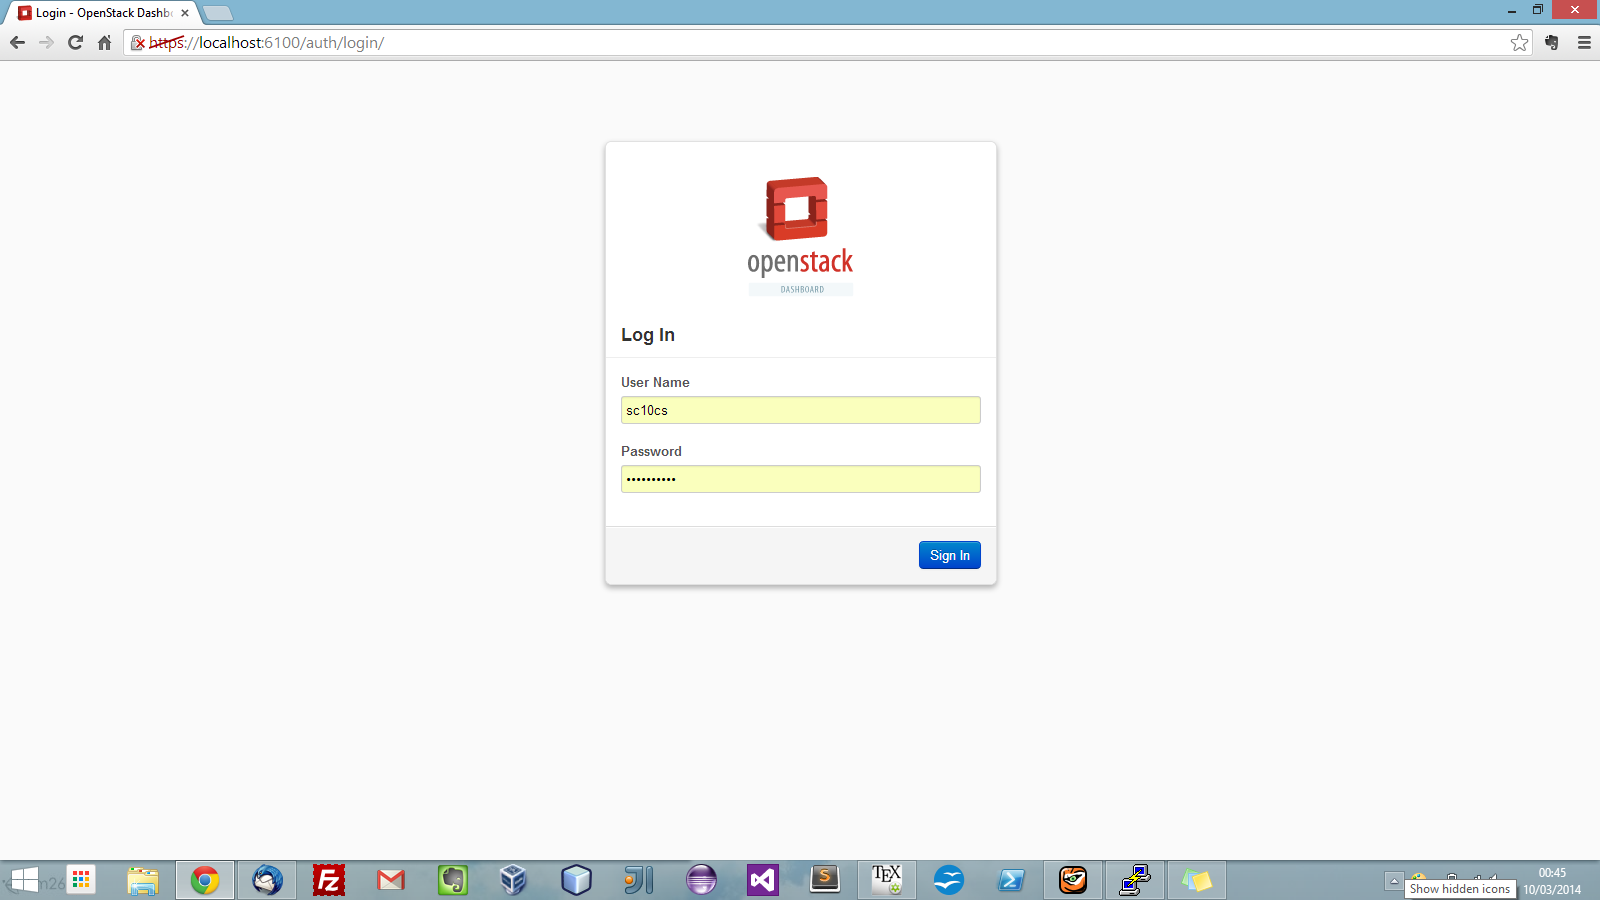
\includegraphics[scale=0.23]{openstack-login}}
\caption{OpenStack Login Screen}
\end{figure}  

\textbf{Step 2: Navigating to the Instance Management View} - Navigating the Dashboard via the various links is very easy, and a good structured view of functionality available. The 'instances' page was accessed by changing project in the 'projects' tag to the sc10cs project, then clicking the 'instances' link on the side panel shown in the below screenshot, which displays the instance management page.
This page contains a navigation panel for various cloud management functions, and a panel on the right to display information based on that navigation. In the case of instances, an empty list of instances with certain information and search functionality can be seen.  
\begin{figure}[H]
\centering
\fbox{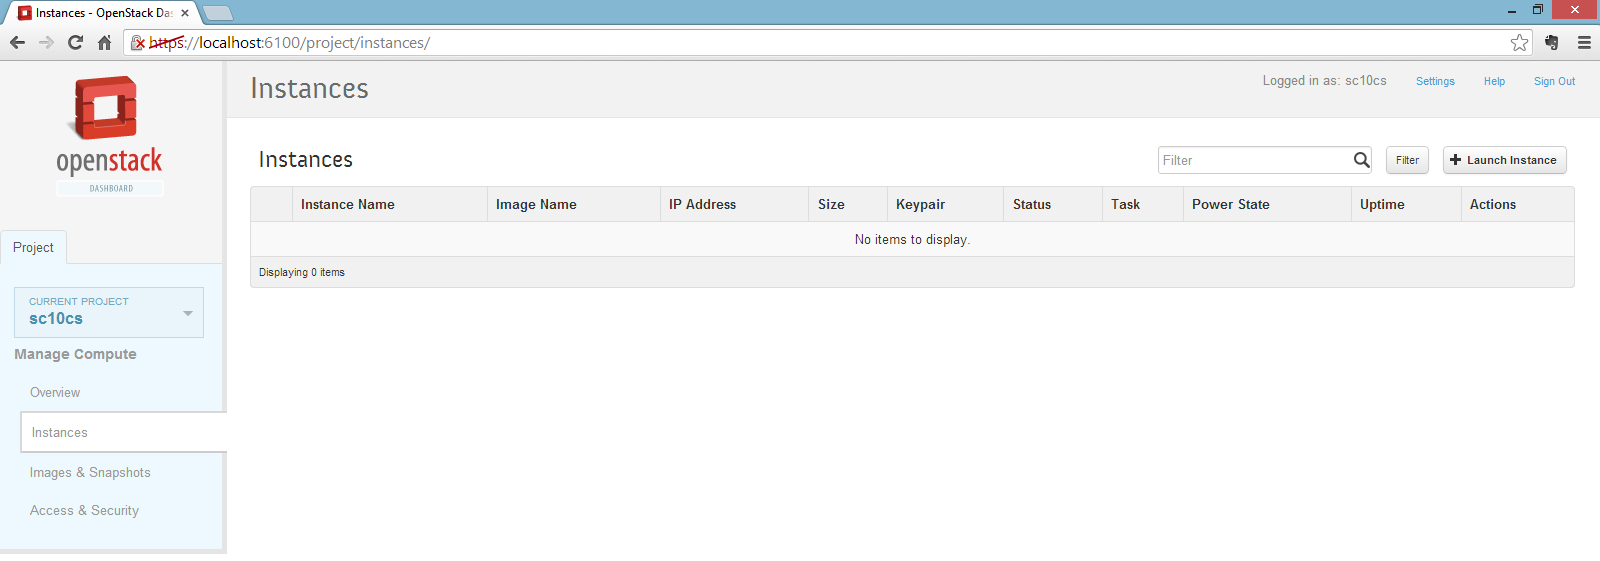
\includegraphics[scale=0.3]{openstack-project-instances}}
\caption{OpenStack Instance Management View}
\end{figure} 
 
\textbf{Step 3: Creating \& Launching an Instance} - The Dashboard UI continues to be very intuitive, and upon clicking the 'Launch Instance' button in the top right of the page, a specialised Instance creation dialog is displayed, shown below. 
\begin{figure}[H]
\centering
\fbox{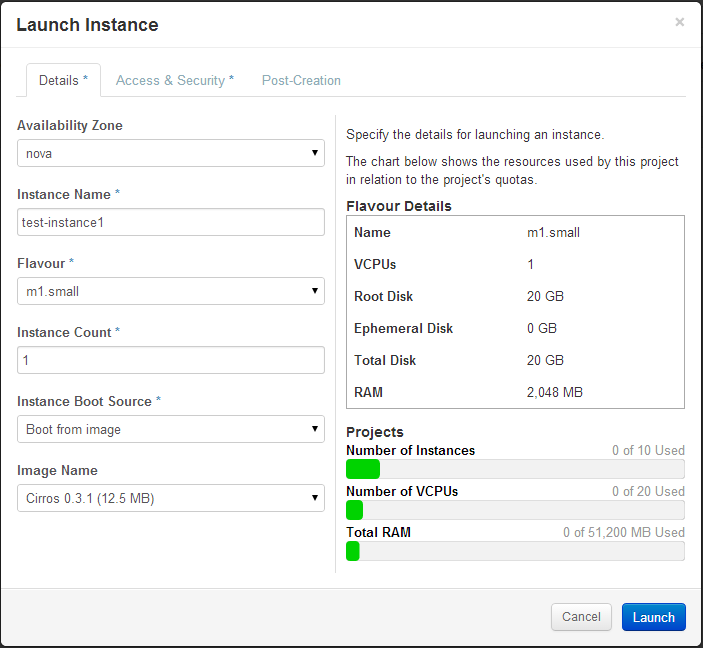
\includegraphics[scale=0.4]{launch-instance-dialog}}
\caption{OpenStack Launch Instance Dialog}
\end{figure}

This dialog allows the user to create a new instance by giving a 'flavour' i.e. a VM size, how much of each resource to allocate to it, and an Image/Snapshot, which act as templates containing deployed software information - these will allow a new instance to be automatically installed and configured by openstack. More options are available in terms of permissions and running post-install scripts. \\

\textbf{Step 4: Checking the Status of the Instance} - Once the launch has been completed, the Web UI almost instantly displays this in the Instances View. Here, certain information can be seen about the instance, including its running status, shown in the below figure:
\begin{figure}[H]
\centering
\fbox{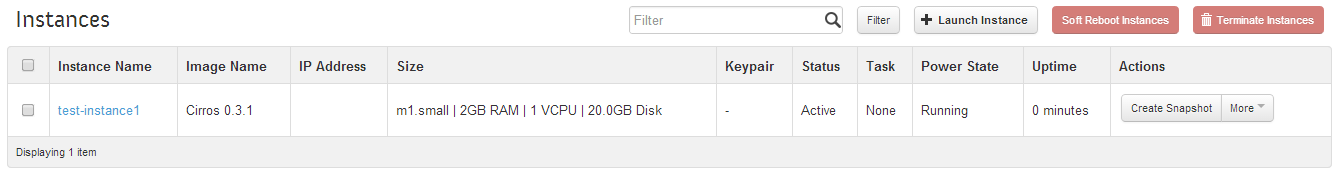
\includegraphics[scale=0.35]{instance-launched}}
\caption{OpenStack Launched Instance}
\end{figure}

\textbf{Conclusion} - 
The Dashboard appears to be an incredibly useful tool. It allowed for quick \& easy authentication through a basic login screen, and simple execution of the task of launching an instance. This tool would be useful for inexperienced users, as it gives a good view of OpenStack functionality, and is very easy to use. Another benefit of the Web Based approach is accessibility; it can be accessed from anywhere with access to the testbed network without logging into the OpenStack machine itself. The main disadvantage of this approach is of course its manual nature - complex tasks may not be suited as they would involve a lot of pointing and clicking. It is my opinion that for my experimentation, smaller, proof of functionality tests would be well suited to execution through the Dashboard.  

\section{Command Line Interface (CLI)}

OpenStack offers a number of Command Line Interfaces, one for each project, which can be used to execute many tasks including Cloud Management \& Information gathering. As the name suggests, this interface to OpenStack is achieved on the Command Line, using a terminal, and using SSH to log directly into the OpenStack machine, testgrid12. The experiment in question will involve use of two main projects, keystone for authentication and the nova for launching an instance. The correct commands must be discovered \& executed in a script, which is provided in this section. To gain a working knowledge of the Command Line Clients associated with OpenStack, I used the official command line reference\cite{openstackcli}.

\textbf{Step 1: Configuring the API Client} - Before any work on the command line could begin, an OpenRC file with information allowing API access was needed. This was accessed through the Dashboard, in the sc10cs project, under Access \& Security -> API access. This file was transferred to the sc10cs account on the OpenStack machine testgrid12 and sourced. It supplies a number of credentials and environment variables which allow access to the CLI. This file is shown below. \\

\begin{figure}[H]
\centering
\fbox{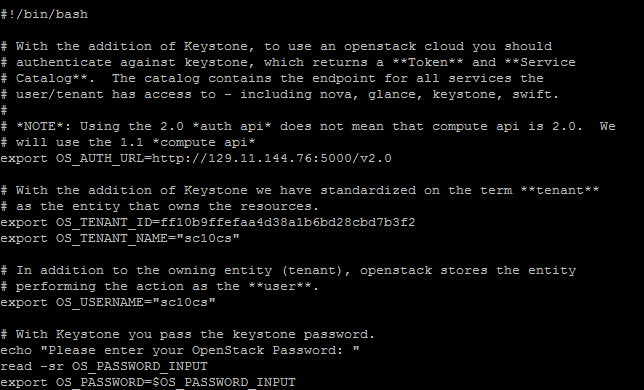
\includegraphics[scale=0.4]{openstackrc}}
\caption{Openstackrc file generated by Dashboard}
\end{figure}


The idea of using a file such as this is that it skips the authentication step of the client process. This information is then readily available to the sc10cs account on testgrid12, and credentials are implicitly included in every command. This greatly simplifies the process of interacting with OpenStack.
The fact that I found this file easy to find out about is a testament to the quality of the official documentation surrounding OpenStack - the information was readily available and easy to access for someone trying to use the CLI.
 \\

\textbf{Step 2: Launching an Instance }- To launch an instance, the nova client's boot command was used. Example boot command usage is as follows:
\begin{figure}[H]
\centering
\fbox{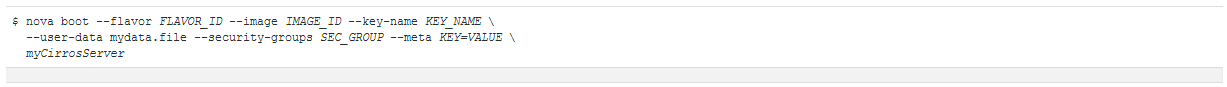
\includegraphics[scale=0.4]{nova-boot-usage}}
\caption{Nova boot usage example}
\end{figure}

In order to use this command effectively, there was a process of using the nova client to obtain certain information about the current system. For example, to find the '\textit{FLAVOR\_ID}', a list of flavors was needed, achieved through using the command '\textit{nova flavor-list}'. The process of obtaining this information as well as image template info and using this to launch an instance is shown below. A scripted version of this is available at the end of this Appendix. The result of the command, shown below, is a table containing status information about the booting instance. 

\begin{figure}[H]
\centering
\fbox{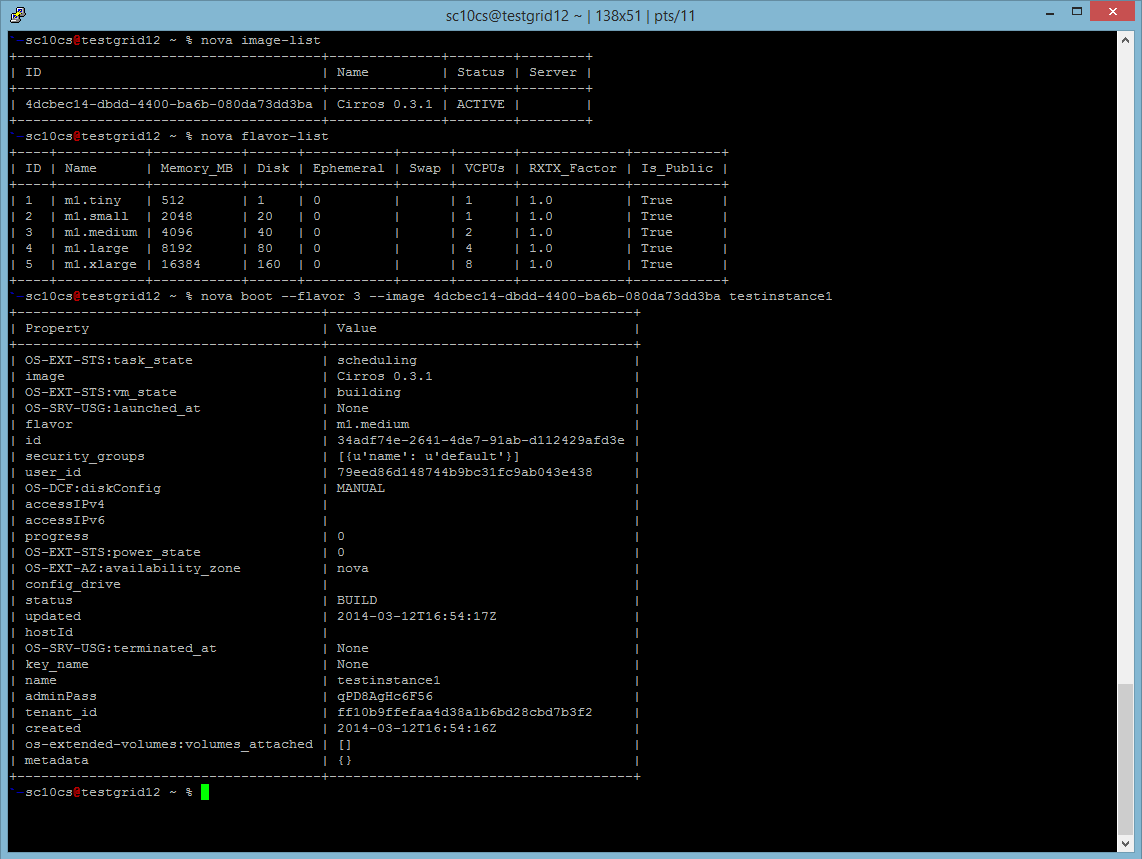
\includegraphics[scale=0.4]{CLI-warmup}}
\caption{Use of Nova to Launch an Instance}
\end{figure}

\textbf{Step 3: Checking the status of the Instance} - Checking up on current images is very simple in the CLI, and only requires one command: \textit{nova list}. The result of this command is a table somewhat similar to the dashboard instances monitor from the first experiment. This table gives the same status information, and is pictured below:
\begin{figure}[H]
\centering
\fbox{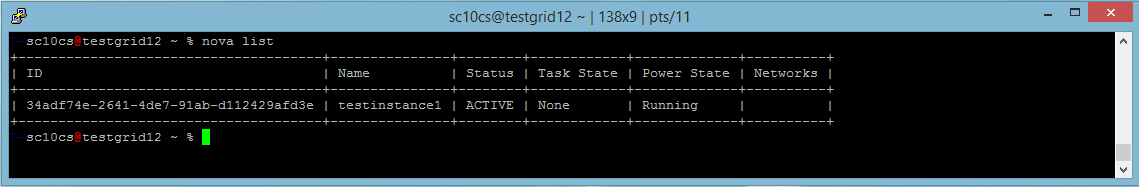
\includegraphics[scale=0.4]{CLI-warmup2}}
\caption{Checking instances with Nova}
\end{figure}

\textbf{Conclusion} - The CLI APIs for OpenStack are a powerful tool. They allow for a wide range of customisation in terms of functionality, and the documentation and response quality surrounding them is of a high standard, meaning that new users could pick them up relatively easily. Another huge advantage of the CLI is the ability to develop automated scripts, especially suited for those tasks which are repeated often and with little variation, for example, a daily status log of instances. This may be useful for some of the practical experiments I plan to execute. There are some obvious disadvantages to this approach, namely the need for configuration of the openrc file and lots of arguments such as tenant\_id which are not intuitive. A second drawback is the need to actually have access to the local OpenStack machine to perform such commands. \\

\textbf{The Script} - The final script of commands used in this experiment to launch and check an instance will be included in my final submission. \\

\section{RESTful Web Service APIs}

RESTful Web Services are APIs exposed over a network through using REST principles. REST, or Representational State Transfer, "\textit{encompasses a simple philosophy for modeling problem domains: “give a URI to everything that can be manipulated by a limited set of operations and let the client software determine the usage metaphor}.”\cite{restoreilly}. Practically, this means each resource is made available with a particular URI, and this is manipulated using HTTP requests which translate to stateless API operations. For example, one may send a POST request with information representing a Server to the server URI \textit{http://openstackint.com/servers}, and this represents the creation of a server. Similarly, sending a HTTP GET request to the same URI may return information about servers. Messages are usually sent in XML or JSON format. More information about REST can be found in the O'Reilly paper on REST\cite{restoreilly}. \\ 

\textbf{Step 0: Setting up Development Environment} - In order to effectively develop experiments using REST Apis, I decided to use the Spring framework\cite{springframework}, an inversion of control framework with REST support, to create clients. This process involved setting up the Eclipse IDE\cite{eclipseide} and using the dependency management tool Maven\cite{maven}. This approach is very popular for REST Clients, although there are alternatives I could have used, such as Jersey\cite{jersey}, which was used in the Distributed Systems Module coursework. 

In order to set up the project, I first installed the Eclipse IDE by downloading a windows executable from \textit{www.eclipse.org}\cite{eclipseide}. Once this was installed, the next step was to create the project. Using Maven, dependencies, such as spring core libraries, are specified in an XML file instead of downloading them manually, and this allows the organised, automated download \& resolution of dependencies at any stage in the development or testing process, e.g. at compile time. An example of one of these files, called \textit{pom.xml}, is shown below. In this project, I used the Spring libraries as well as the Jackson JSON processing library\cite{jackson} for converting Java objects to and from JSON format, the message format used for Openstack's REST APIs.  

\begin{figure}[H]
\centering
\fbox{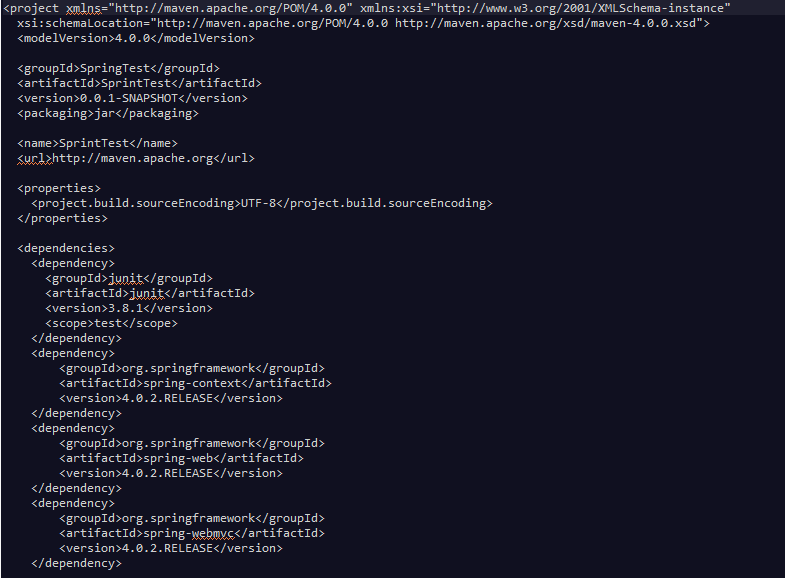
\includegraphics[scale=0.35]{pomxmlexample}}
\caption{Example project pom.xml maven dependency file}
\end{figure}

As part of setting up this project, a lot of research into how the Spring framework, maven \& Jackson work was required. Due to this, the first main point of consideration I noticed was that, although REST clients can be created through basic HTTP request tools in any programming language, to create a professional and effective REST client, i.e. using Spring or Jersey, there is a lot of prerequisite knowledge, compared to using the Dashboard or the CLI. I will briefly introduce the Spring Framework and Jackson in the next steps. \\

\textbf{Step 1: Research Openstack REST APIs} - Before actually developing clients with the tools I had chosen, it was important to first understand the workings of the Openstack REST APIs. For this, I used the official API reference\cite{openstackdocs} along with other sources found on the internet, which will be introduced as they are referenced.  Due to the nature of the first experiment, I focussed on the Keystone \& Nova APIs, as well as formulating a process by which to test out a REST API for further experiments. \\

The first step in accessing an Openstack REST API was figuring out how to actually access the API endpoints, i.e. the Base URL to send requests to. Intuitively I knew that \textit{testgrid12} would be the network resource forming the first part of this URL, accessed over HTTP. From this point, I discovered in the Openstack API refs that a different port is allocated to each service, e.g. Keystone, Nova. One disappointing aspect of the Openstack Documentation is that the port for each service was very difficult to find out, which seems strange as this is vital information. I found the port for each service from scouring the Q \& A board for Openstack\cite{openstackports}, and some of these are displayed below:

\begin{figure}[H]
\centering
\fbox{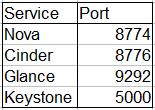
\includegraphics[scale=0.5]{serviceports}}
\caption{Ports for given Openstack services\cite{openstackports}} 
\end{figure}

Once these were accessible, I needed to find a way of sending test requests to these endpoints in order to validate them, and make sure they are functional. Due to requests being made using existing HTTP technologies, there are a number of ways of doing this. For example, a GET request is sent just by putting the URL into a browser's address bar. In this way we can access the keystone API's base URL, which gives API information in response to a GET request, as shown below:

\begin{figure}[H]
\centering
\fbox{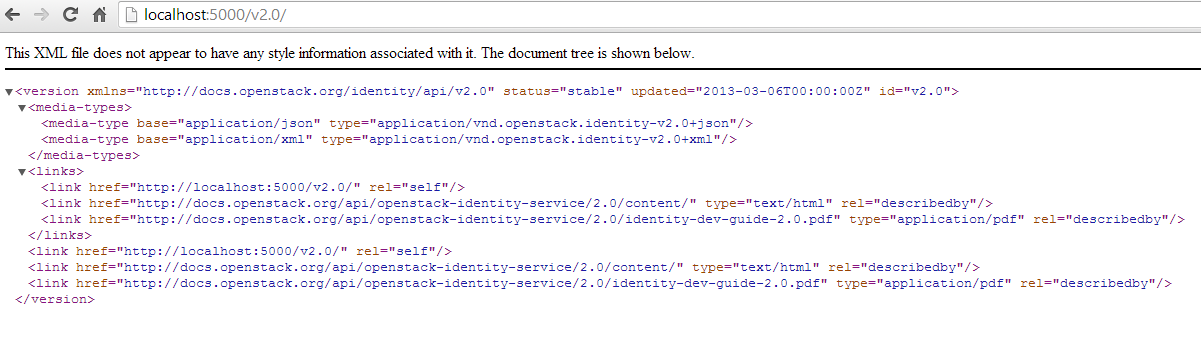
\includegraphics[scale=0.4]{identitybrowserget}}
\caption{Accessing the Keystone Service through a browser} 
\end{figure}

Similarly, the \textit{curl} command can be used to send requests, as shown below: 

\begin{figure}[H]
\centering
\fbox{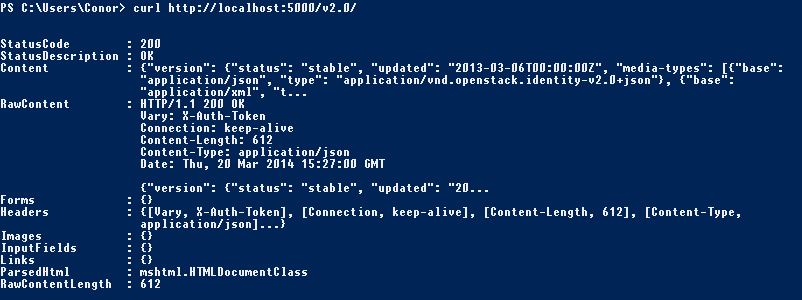
\includegraphics[scale=0.4]{identitycurlget}}
\caption{Accessing the Keystone Service through \textit{curl}} 
\end{figure}

Both of these approaches are valid for basic requests, but for my validation of requests, I used a tool called 'Advanced Rest Client'\cite{advancedrestclient} available as an application on the Google Chrome App Store\cite{googleapps}. This allows for customisation of requests including advanced features such as headers and several message types, including raw JSON. An example of the easy to use Web UI for ARC is shown below: 

\begin{figure}[H]
\centering
\fbox{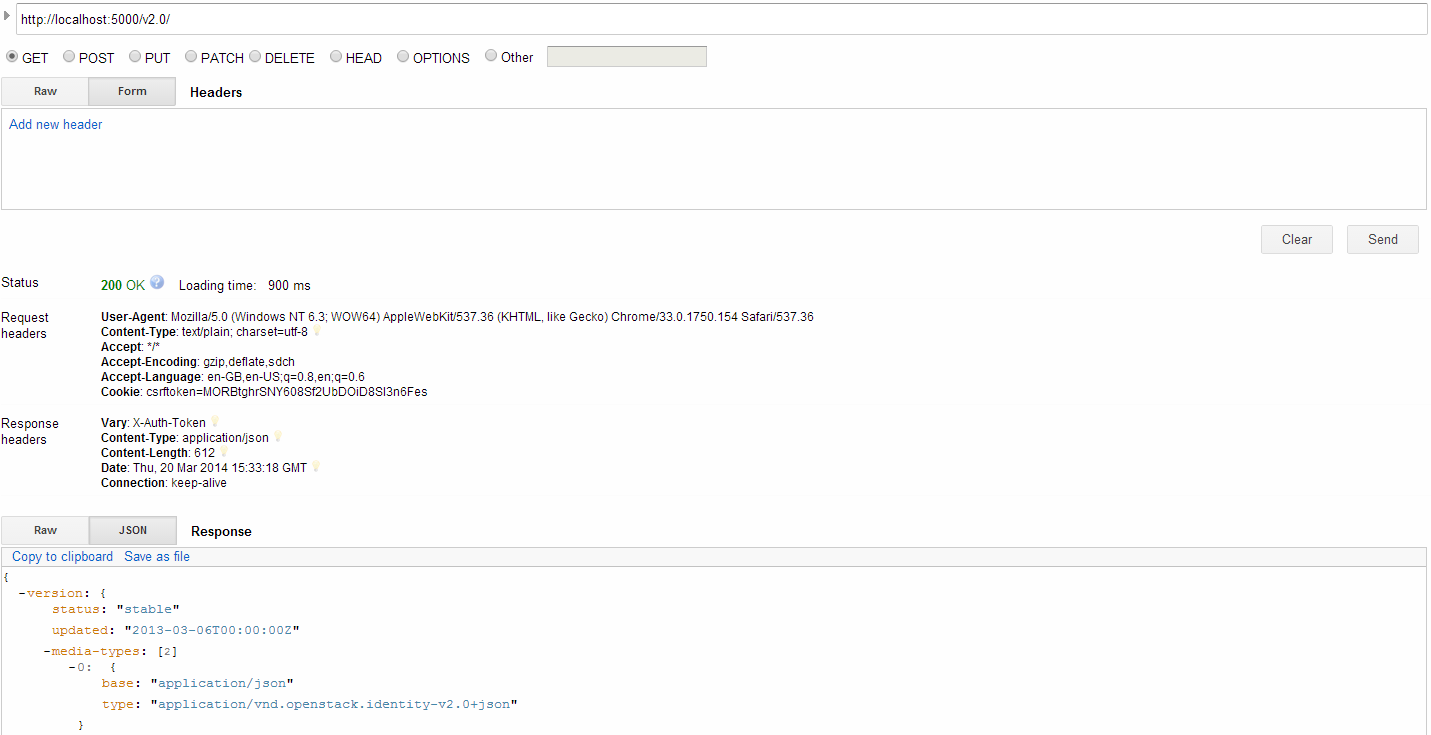
\includegraphics[scale=0.3]{advrestclient}}
\caption{Using Advanced Rest Client to interact with Keystone} 
\end{figure}
 
At this point, I had a way of simulating a rest client to step through the HTTP requests required for the first experiment, as well as the development tools in place to automate the firing of these requests and create a programmatic client. \\

\textbf{Step 2: Developing the Rest Client} - In developing the REST Client for experiments, there were 2 main parts of the work. The first of these was to develop clients for each Openstack service, and some programmatic structure for writing experiments without repeating large parts of the logic in each experiment. Object Oriented Design was used to achieve this goal. Secondly, once the structure of the program was in place, it was time to discern which requests to send to which URIs in order to achieve the aims of the experiment, to launch an instance. Both parts of the work will be described below. \\

\textbf{\textit{Step 2A: Designing \& Implementing Project Structure}} - The structure of the project was based mainly on requirements of the project. The main aspects of the project required were:

\begin{itemize}
\itemsep0em
\item A way of injecting OpenStack configuration (e.g. base uri, ports, user \& password) for different setups. 
\item A way of choosing a number of experiments to run, similar to injecting config files. 
\item A way of easily writing experiments to hook into the experiment runner. 
\item A number of client-side representations of services such as Keystone identity service, to be consumed by experiments. 
\item Some way of reading and writing JSON messages to communicate with REST APIs. 
\end{itemize}

The first requirement, the ability to inject configuration into the application, is something very easily achieved through the use of Spring functionality. Spring allows for XML files to be used to define properties of 'Beans', which are Java Objects with properties determined by these XML files. This is a form of 'Dependency Injection', where values are handed to objects from some outside source, rather than being hard-coded, allowing for less coupled and more flexible applications. For example, in the case of OpenStack configuration, a different XML file can be loaded for different OpenStack installations, users, etc. Every XML bean definition will have a corrsponding class, in this case, \textit{OpenstackConfig.java}, which is populated by the bean definition. These populated objects are loaded into an \textit{Application Context}, through which they can be accessed. The bean definition used for the TestBed can be seen below, along with the corresponding Java class:

\begin{figure}[H]
\centering
\fbox{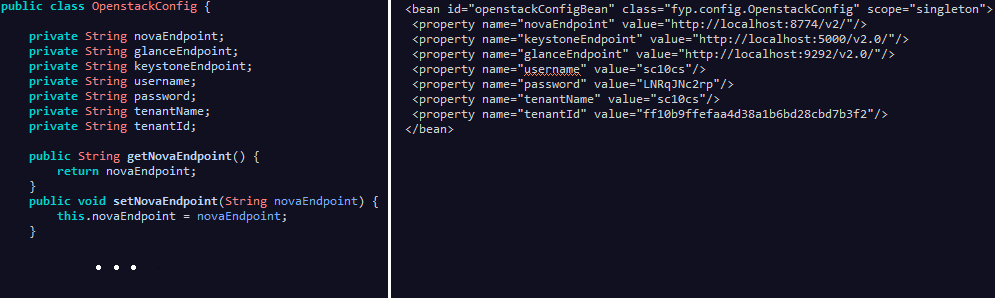
\includegraphics[scale=0.45]{configbean}}
\caption{OpenstackConfig class \& Corresponding Bean definition} 
\end{figure}

Next, to satisfy the requirement to have some way of creating new experiments and a way of running them, I created an abstract class \textit{Experiment}, with the intention that every Experiment would be a subclass of this class, and would need to implement methods to set up, run and tear down the experiment, making it easily executable by a second \textit{ExperimentExecutor} class. Finally, in order to tell the Executor class which experiments to run, a new Bean was defined, based on the java.util.ArrayList class, containing a list of class names for different experiment subclasses. This is loaded into the Application Context by the ExperimentExecutor and each is executed. Below, a class diagram representing what has just been described is shown.

\begin{figure}[H]
\centering
\fbox{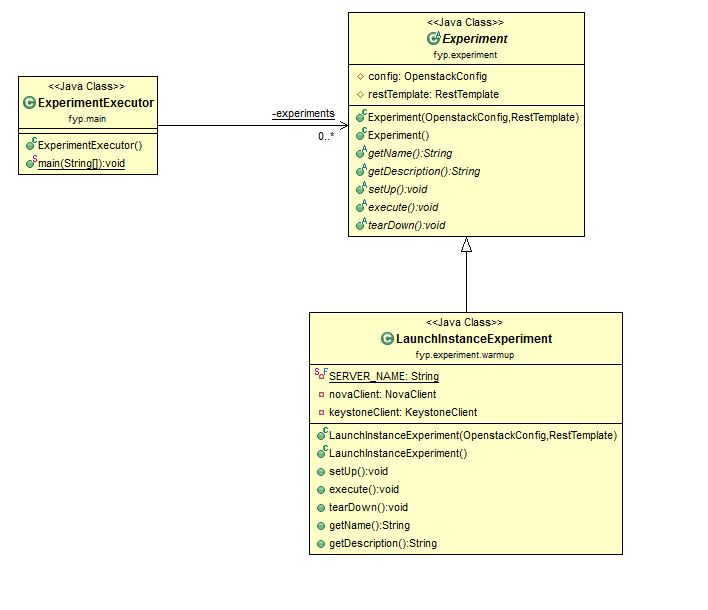
\includegraphics[scale=0.4]{experimentclassdiagram}}
\caption{Class Diagram for Experiment execution} 
\end{figure}

The next requirement, a number of client-side representations of openstack services, was achieved through basic OO abstractions, in the form of interfaces, one for each service, detailing the functionality offered by this service. This is similar to the concept of a proxy class introduced in the Distributed Systems module concerning Java Remote Method Invocation; it is a local version of the functionality which marshals and passes messages. The main difference is that each of these interfaces will be implemented with logic which will perform REST web service interaction with Openstack. The following class diagram demonstrates this use of client interfaces: \\

\begin{figure}[H]
\centering
\fbox{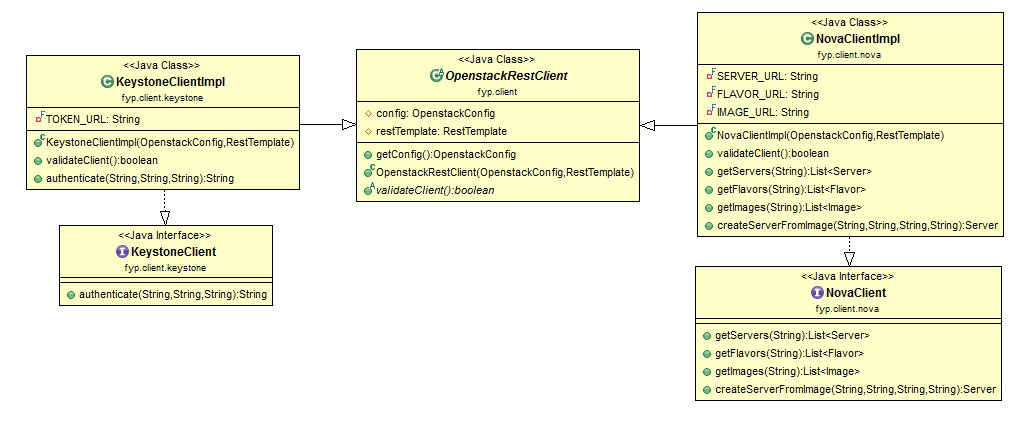
\includegraphics[scale=0.4]{clientclassdiagram}}
\caption{Class Diagram for Openstack clients} 
\end{figure}


Finally, the implementations of the aforementioned interfaces require some way of reading and writing JSON messages to communicate with REST APIs. For this, I used Jackson, a JSON processor with the capability of mapping Java Objects to and from JSON representation. This means that, as long as classes are created to represent data mapping to requests and responses with Openstack, the JSON mapper will implicitly generate and parse JSON. An example of a java class and its JSON counterpart can be seen below.

\begin{figure}[H]
\centering
\fbox{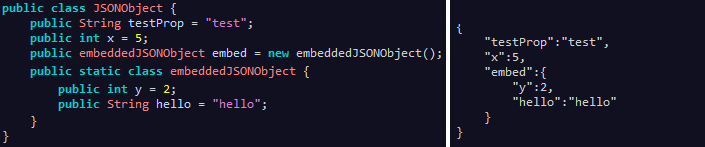
\includegraphics[scale=0.5]{jsonrequestclass}}
\caption{Java request class and mapped Jackson JSON representation} 
\end{figure}

\textbf{\textit{Step 2B: Implementing Experiment Client Functionality}} - In order to execute the first experiment, the correct functionality from both Keystone and Nova clients was needed. The operations required are similar to those required for the CLI experiment, and were researched using the official REST API references for each Service. \\
Firstly, for authenticating with keystone, a POST request to \textit{http://testgrid12:5000/v2.0/tokens} containing user credentials was required, returning a session token to be sent in subsequent requests. To perform REST requests with spring, the \textit{RestTemplate} class is used. A simple call to the \textit{postForObject} method, used in conjunction with the Jackson object mapper, deals with sending and receiving from the Keystone API. The code to do this is shown below:

\begin{figure}[H]
\centering
\fbox{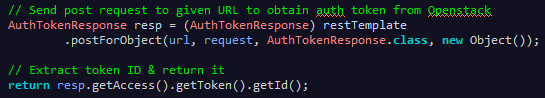
\includegraphics[scale=0.5]{tokenauth}}
\caption{Authenticating a session with Openstack via REST} 
\end{figure}

Once this was authenticated, four more operations were required to be implemented; three of these were relatively simple GET requests to obtain information about which instances, flavors, and images are available. The final operation was a POST request which actually creates and launches a server instance. \\
For any type of request which manipulates openstack resources, an authentication token from the previous request is required. For this reason, the \textit{HttpEntity} class was required as opposed to a simple method representing an HTTP request. An example of this, to create servers, is shown below, encapsulated in a method on the NovaClient interface:

\begin{figure}[H]
\centering
\fbox{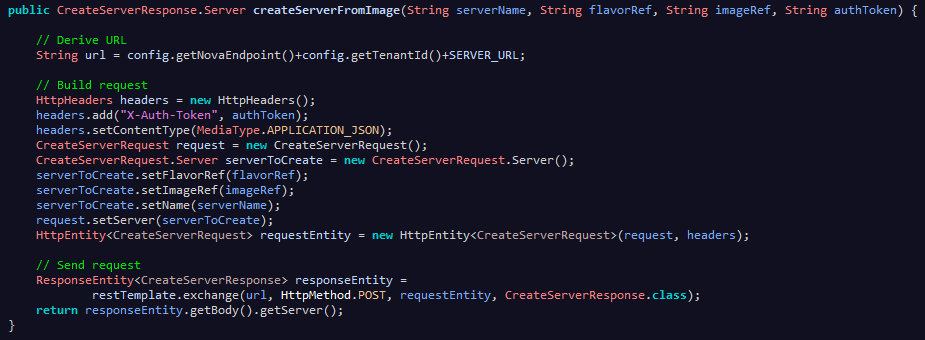
\includegraphics[scale=0.5]{createservercode}}
\caption{Method to create a server on Openstack via REST} 
\end{figure}

Once this was completed, the Experiment could be written. The experiment consists of a number of steps. Firstly, servers, flavors and images are listed from the server. Next, a server instance is created. Servers are then retrieved again, to ensure that launching the instance was actually successful. The code for executing this experiment is shown below. 

\begin{figure}[H]
\centering
\fbox{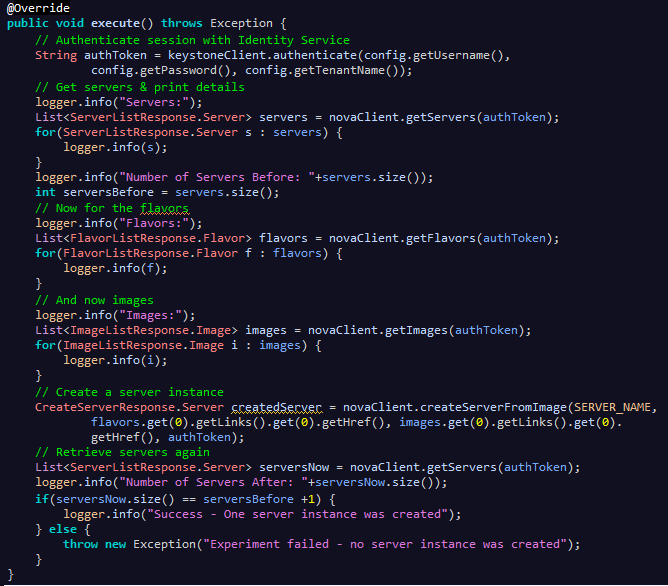
\includegraphics[scale=0.5]{launchinstanceexecute}}
\caption{Experiment to Launch an instance via REST} 
\end{figure}

\textbf{Step 3: Executing the Experiment, Logging results}

Executing the experiment was performed from Eclipse, simply by choosing the option to 'Run as Java Application'. To log results, the Apache Logging tool Log4j was used\cite{log4j}. In the Log4j properties file, included in the submission accompanying this project, a log file is specified to write to as well as to the Eclipse Console (standard output). The output to this log file, from running the experiment, is shown below:

\begin{figure}[H]
\centering
\fbox{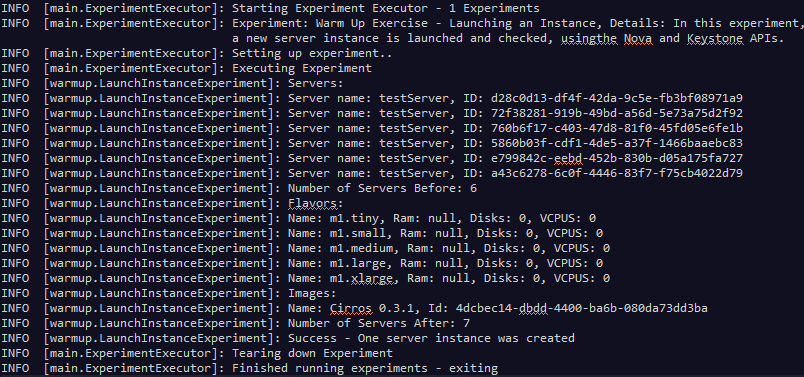
\includegraphics[scale=0.5]{executewarmup}}
\caption{Results of running warmup experiment via REST Client} 
\end{figure}
  
\textbf{Conclusion}  

The OpenStack REST APIs are an incredibly powerful automation tool. They allow the use of Object Oriented principles, or any other structured programming paradigm, through the ability to develop clients in any programming language. This means that clients can be as simple or complex, and similarly as developed as the user wishes. This flexibility makes REST APIs a very useful tool for larger automation tasks, perhaps those which need to be flexible to change and further development, or are complex enough to benefit from the plethora of debugging \& development tools available to modern programming languages.  

One huge advantage of these APIs is the ability to remotely access each individual project on a different port; in the case of the Command line, a direct login to the OpenStack machine is required, and this can cause certain problems with security - in the case of REST, ports can be exposed to easily give access to outsiders. The fact that this runs over HTTP \& HTTPS, very reliable and secure protocols, is an added bonus. 

Another feather in the cap of the REST APIs is the level of documentation available; OpenStack's official docs, referenced in this section, are very informative, and give a good detailed overview of how to use the API. Tools such as the Advanced Rest Client \& curl make testing this out very easy. Each project, being on its own port, is very nicely separated, and it is easy to see from the client side which project or component is being interacted with - useful information for a client considering a change in configuration, for example. 

There are some downsides I spotted from using the REST APIs. Firstly, clients with any real automated capability are rather difficult to develop, and to really get the benefits of REST over, for example, the CLI, a programming language, and not something like curl, should be used. In many languages, due to the need to parse and generate JSON messages, this can get rather complicated, and in the case of Java, means a lot of 'boiler plate code' to map messages to Java objects. \\
Another huge issue I had was the tracking of jobs. Often, when asynchronous jobs are being performed, a Task or Job is returned, allowing the querying of the state of a job. This is not the case for OpenStack as far as my research has shown, and instead, problems can be caused when there are delays to jobs being completed. For example, deleting a Server takes a few seconds after the request has been sent and a response returned, and so if a list of servers is retrieved before this delay, the server will still appear. This of course could cause many automation issues. 
One other issue was with the use of JSON to represent Objects. Often, there would be multiple representations of the same OpenStack 'entity', such as an Image, or a Server. The problem was, in different contexts, different representations of these would be returned, and this can be difficult for a client to handle, without massively overloading the names of objects. Having 4 different 'Server' classes can cause a lot of confusion! An example of this from the provided source code is the class Server.class, and the class ServerInfo.class. ServerInfo is a different representation of a server in OpenStack, providing less information than Server, which is the response from getting all details of a Server, i.e. a 'full' representation.   
 
  
\section{Experiment Conclusion - Comparing Interfaces}

Provided below is a simple table outlining the advantages and disadvantages of each interface to OpenStack, based on my usage of each in this experiment:  

\begin{figure}[H]
\centering
\fbox{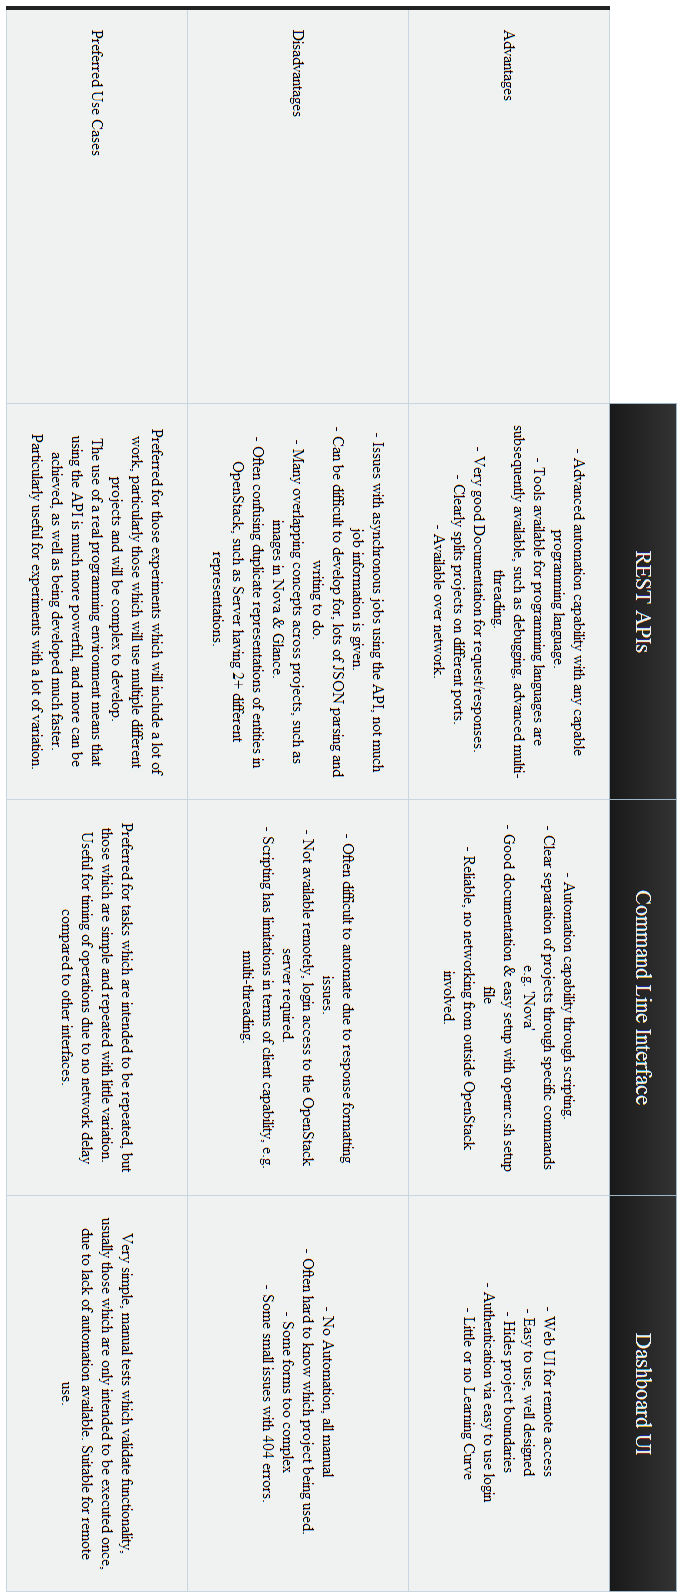
\includegraphics[scale=0.5]{interfacecomparison}}
\caption{Comparison of each interface to OpenStack} 
\end{figure}